\documentclass[thesis.tex]{subfiles}
\begin{document}
\chapter{Background}

\section{The mobile ecosystem}\label{sec:mobile-ecosystem}

This dissertation talks about the policies surrounding \emph{mobile
ecosystems}; but what, precisely, do we mean by the \emph{mobile
ecosystem}?  Succinctly when we refer to the mobile ecosystem we are
referring to \textbf{the interactions surrounding the use of smart
phones and tablet computers}.  Figure~\ref{fig:mobile-ecosystem} shows
some of the relationships between devices, their users and their
preferences, the stores, companies and all these principal's
policies. Users have phones or other mobile devices.  They may own
personal devices or have a company one.  They may have their own
preferred ways of using the device, or they may be subject to policies
written for their employer.  They download apps, written by developers
from app stores, all with their own policies and some of the stores
may delegate some aspects of their quality control to external vetting
software.  Even just describing these aspects of the mobile ecosystem
\autoref{fig:mobile-ecosystem} is quite complex.

To fully understand the scale of the mobile ecosystem, however, it is
best to describe some of the history surrounding it.

\begin{figure}
  \centering
  \includegraphics[width=\linewidth]{figures/mobile-ecosystem.png}
  \caption{Interactions between surrounding the use of mobile devices.}
  \label{fig:mobile-ecosystem}
\end{figure}

\subsection{Mobile devices: the story so far}

Some of the earliest mobile devices were the \acp{PDA} devices of the
early 90s.  The earliest devices, such as Apple's Newton, were
portable miniature computers designed to store personal information,
calendars and notes.  Developers could even program additional apps
for them (in the case of the Newton using Apple's Dylan language).  At
the time mobile phones were just portable telephones, but starting
with the IBM Simon in 1994 these devices started to have some of the
functionality of the \ac{PDA}, becoming what would later be called a
\emph{smart phone}.  The big advantage of these early smart phones
over the \ac{PDA} was they had a telephone connection.  The earliest
devices allowed their users to access email and fax, as well as
managing personal information.  The early smart phones were somewhat
underpowered compared to the \ac{PDA} devices so both continued to
develop alongside one another, and started to become more affordable.

In 1998 the Symbian OS was released.  Developed by Psion (who made
\acp{PDA}), and Motorola, Ericsson and Nokia (all phone
manufacturers).  By the early 2000s it would start to become the
dominant smart phone OS.  These devices could install apps, written in
C++ or Java (if the phone supported JME). They had cameras, could play
music. They even had early malware which would illicitly send texts to
premium rate numbers.  They were the forebears of the \emph{modern}
smart phone.
They were also starting to become affordable, with the lowest end
models starting to being affordable by children and
teenagers\footnote{If you saved up for what seemed like
  forever$\ldots$}.  Devices like Nokia's N-Gage were marketed directly
towards these younger users and featured games users could buy for
their devices.

In the mid-2000s we first start to see the mobile
ecosystem proper.  We have users with different devices, downloading
apps from different sources (some pirated).  These devices
contained personal information of the \acp{PDA}, but also photographs
and music.  Users could browse the web, and send each other pictures.
With increasing amounts of personal information malware authors
started to take note.  In a blog post from 2006 for Symantec, Chien
noted~\cite{eric_chien_spyware_2006}:

\begin{quote}
  ``While threats exist and are actively spreading, we are probably
  still years away from the situation we have with the Microsoft Windows
  [$\cdots$] We have already seen spyware applications for mobile devices
  (e.g. Spyware.Flexispy) that can monitor activities on the mobile
  device and then send them to a remote server. [$\cdots$] Just as
  worrying is the fact that the adware market is just beginning to take
  notice of mobile devices. Already some Bluetooth advertising schemes
  have been tested, where a bus stop is outfitted with a device that
  just spams out messages via Bluetooth.

  [$\cdots$]
  
  So, while worms and Trojans already exist for the mobile
  platforms, spyware and adware applications are just now gaining a
  foothold in the mobile device space. Spyware and adware pose a
  potentially large security issue in the near future, as the companies
  that produce such applications are less affected by the natural
  limiting factors.''
\end{quote}

In 2008 Apple released the first iPhone, and shortly after Google
released the Android OS.  Symbian would release its final version in
2012, with Android as the dominant OS on most devices.  These
operating systems differed from past efforts, and conventional desktop
OS, in that they were far more controlled than previous systems.
Apple's devices could not run code that Apple had not signed or
install software from outside of its App Store, which Apple
controlled.  Android devices offered a similar app marketplace, but
where there seemed to be less checking of individual
apps~\cite{oberheide_dissecting_2012}. Whilst Android users could
install software from other sources, the option was hidden by default.
As well as restrictions to software, these devices were also better
protected.  Devices no longer had an all powerful \emph{root} account.
APIs were provided that restricted malicious behaviors.  One example
was stopping SMSs being sent programatically to premium rate accounts;
essentially ending a monetization technique that had been prevelent in
malware before. 

Mobile devices stored a large amount of personal data about their
users.  They contained address books, records of phone calls, and GPS
logs of where their users had been.  With iOS and Android user's
became more aware about privacy on their devices, in part because of
increased media coverage of privacy issues.  A survey in 2012 by
Chin~et~al{.} found that users were more concerned about privacy on
their mobile devices, than on their
laptops~\cite{chin_measuring_2012}. Users of a smartphone were more
likely to install an app that came recommended from a friend, was
popular or was free.  To subsidize the cost of producing free apps,
and to better understand how users used their apps, some developers
added adware and tracking libraries to their apps.  These libraries
accomplished a variety of tasks ranging from crash and error tracking,
to collecting personal data to be sold to advertisers to subsidize the
app's price~\cite{seungyeop_han_study_2012}.

This dynamic between users who were increasingly concerned about their
privacy and apps which were increasingly privacy invading, lead many
to argue that the mobile device operating systems needed better
controls for what data and permissions an app could
have~\cite{leontiadis_dont_2012}.  Many different schemes were
suggested to fix this and provide finer privacy
controls~\cite{jeon_dr._2012,beresford_mockdroid:_2011,conti_crepe:_2010,backes_appguard_2013}
(some of which will be described further in
\autoref{chap:related-work}).  In general, however, users did not
really understand the how app permissions
worked~\cite{felt_android_2012}.  By 2017 (and the present day) iOS
and Android had settled on a model where user's were asked by their
devices if an app could access certain data when it first requested it
and then the user could revoke that decision later if they wished.
Despite the present Android permissions model being \emph{ask on use},
a large number of older Android devices are still being used.  In June
2016 only 10\% of devices used the latest version of Android, with
around 5\% using a version more than five years old
(\autoref{fig:android-versions}).  In contrast 79\% of iOS devices use
the latest OS, 16\% use the previous version and only 5\% use anything
older~\cite{apple_app_2017}.  The greater fragmentation of the Android
versions has been attributed to the greater number of Android device
manufacturers each with their own update mechanisms as compared to
with iOS where Apple exclusively control and update all devices.

\begin{figure}
\centering
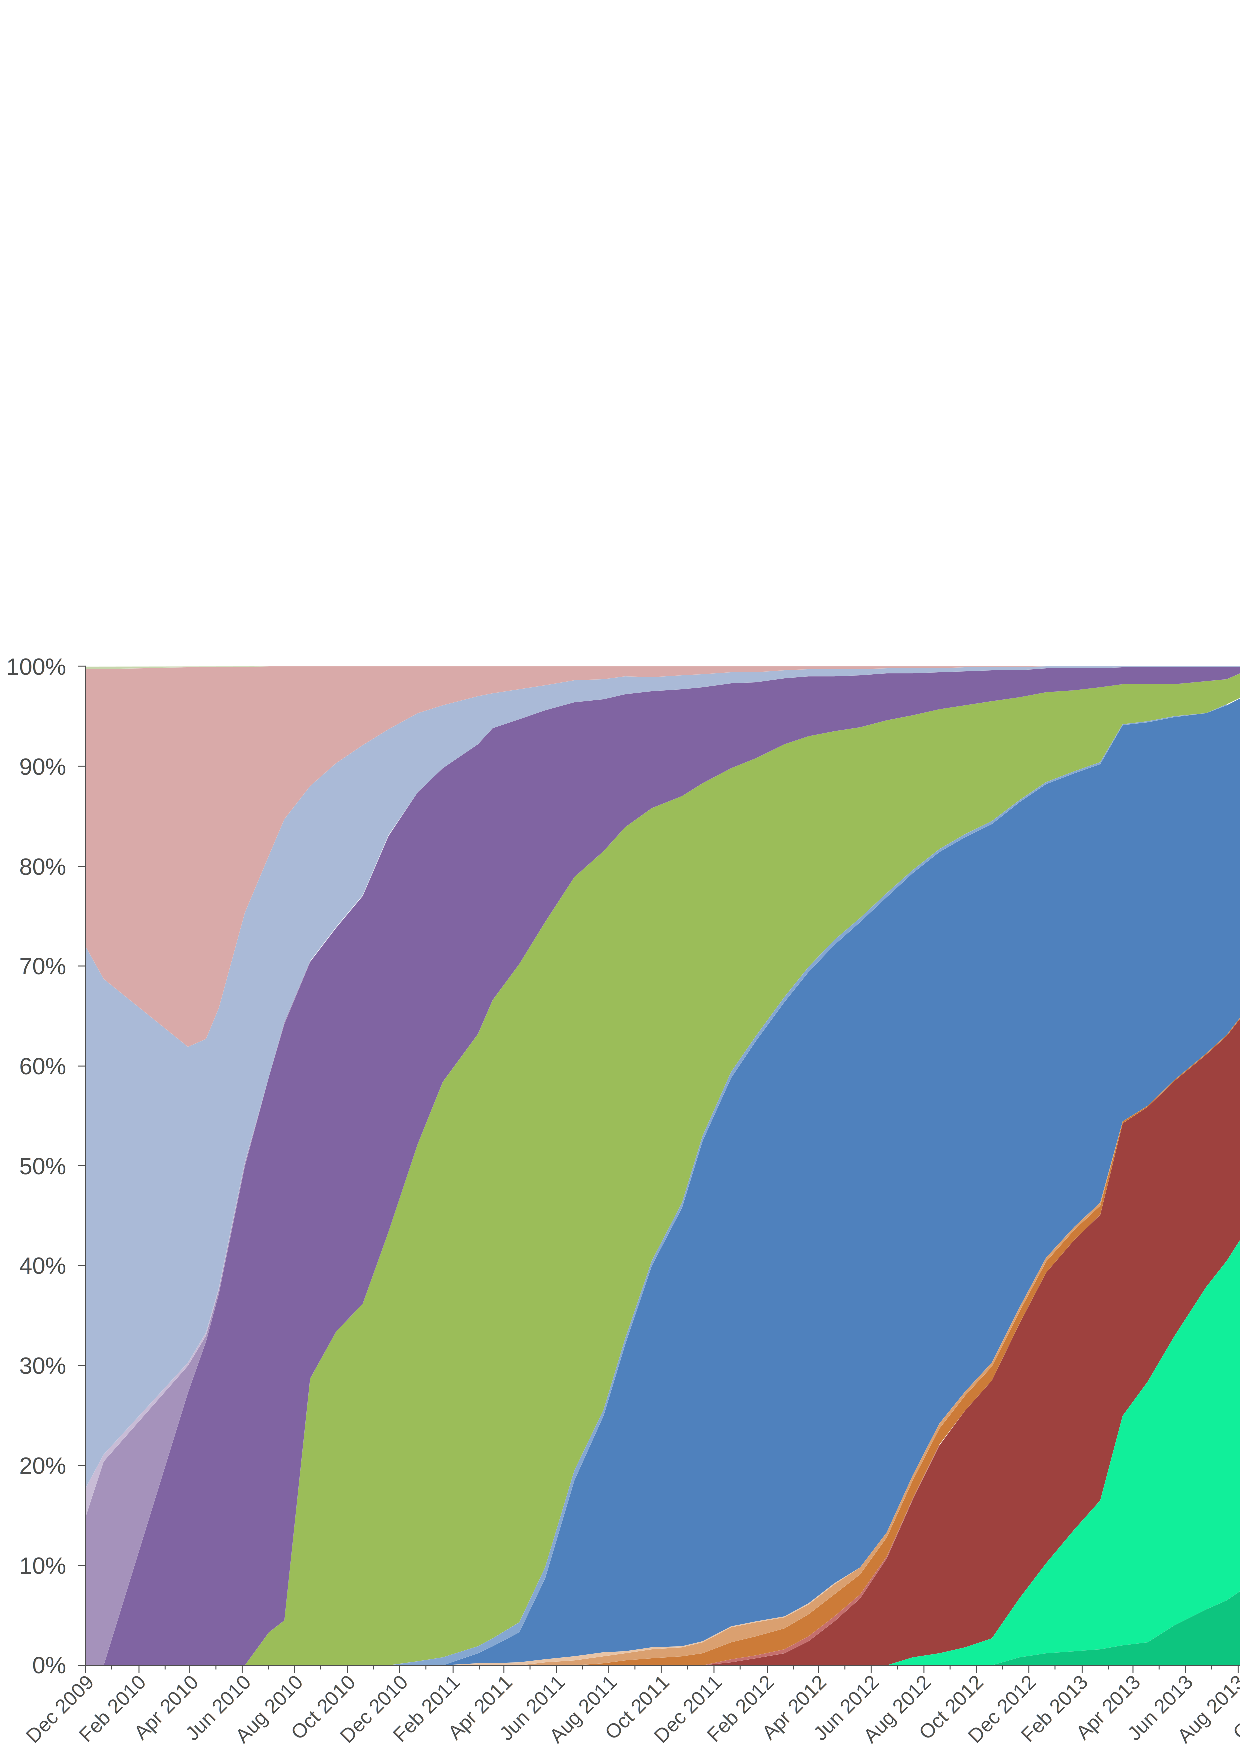
\includegraphics[width=\linewidth]{figures/android-versions.pdf}
\caption[Historical Android version's distribution.]{Historical Android
  version's distribution~\cite{erikrespo_android_2017}.}
\label{fig:android-versions}
\end{figure}

Mobile devices became more ubiquitous, and \acp{PDA} reappeared now
called \emph{tablets} or \emph{iPads}.  These devices were identical
to the smart phones, but larger and they generally did not have a
cellular data connection instead using wifi. They could not send
texts or make phone calls but a shift away from traditional SMS and
cellular phone calls to internet backed communications such as
WhatsApp, iMessage, Skype and FaceTime meant these devices were
essentially interchangeable with smart phones.

Advances in secure co-processors meant that mobile devices were even
more capable.  Banks allowed users to link their devices to their bank
accounts and use their device, or even the new \emph{smart watches} as
a debit card.  This quickly became a common and ubiquitous payment
method quickly with even street vendors, who hadn't taken cards
previously, accepting contactless payment via a mobile device.  The
separation of cryptographic operations from everyday computing with
secure co-processors and secure enclaves (such as TrustZone) lead to
significantly improved security.  Keys could be isolated from the
entire mobile OS, allowing for increased trust mechanisms.

Mobile devices gained the ability to collect increasingly personal
information.  Smart watches recorded and shared a user's pulse with
others. Mobile health apps were made to track and monitor medical
conditions. In the US, the \ac{HIPAA} required that healthcare
providers transmited medical information securely, but many apps had
basic security problems~\cite{fahl_why_2012}, and many of the
healthcare apps did not handle the medical information
securely~\cite{knorr_privacy_2015}.

\subsection{The Mobile Ecosystem and the need for Policies}

With mobile devices becoming increasingly capable and managing ever
increasing amounts of information there is a need to manage how the
devices behave.  As users become aware of the privacy implications of
their devices, they express preferences about which apps they want to
install~\cite{sadeh_understanding_2009}, even if they do not follow
through on their preferences~\cite{hallett_apppal_2016}.  Employees
now bring their mobile devices to work and use them to access company
email and documents.  In response to this companies publish mobile
device policies that describe how the devices should be used within
the company.  They may also use \ac{MDM} software to enforce the
policies.  If a company wishes to use an app for business purposes
there may be regulation they need to follow, such as \ac{HIPAA}.

These policies vary in terms of formality.  A user may never write
their privacy preferences in a formal language, but they may make
decisions guided by them.  For example which apps to install and which
to avoid.  They may make decisions based on what their friends have
told them, or what a review said about the app.  By describing the
policy in a formal language we can start to express the policy more
rigorously.  We can start to make comparisons between users, and with
rules for checking the policy start to help the user to make decisions
more accurately, or measure the extent a user follows their stated
policy~\cite{hallett_apppal_2016}.  

A company looking to control the mobile devices their employees bring
to work might write a \ac{BYOD} policy.  They might also use \ac{MDM}
software to control some aspects of their devices.  The company might
write these with varying degrees of formality but often they are
written using natural language.  This adds vagueness and can lead to
confusion as to how a policy should be implemented.  Using formal
languages we can model the policies precisely, helping clarify their
meanings and make precise comparisons between different policies.  We
can tie the rules in the \ac{BYOD} policies to the \ac{MDM} tools used
to implement them.

If a company needs to use apps which conform with a policy such as
\ac{HIPAA} they could use static analysis tools to check for some
aspects of the policy.  Perhaps the company might use
Mallodroid~\cite{fahl_why_2012} to detect when data is sent
unencrypted.  It is important, however, not to confuse the tools and
techniques we might use to implement parts of a policy with the end
goal of ensuring that the policy is followed.  A formal language that
lets us tie the policy to its implementation can help show how the
policy is checked.  It lets us see what rules from the policy are
checked for by which tools, and identify gaps where the policy is not
being checked.

When describing how mobile phones had evolved, we described how we
arrived with two main operating systems for mobile devices: iOS and
Android.  The trust models in the systems differ, as do the
assumptions about what an app can do when running on each system.
There are also similarities.  iOS and Android (from Android M) have a
similar permissions system for apps.  When people make comparisons
between them, however, the differences are often vague.  iOS is a
\emph{walled garden}.  Android is \emph{more open}.  Again, by using
formal languages we can start to make comparisons that are precise and
show the differences clearly.

We need an authorization logic for mobile ecosystems.

\section{SecPAL}

SecPAL is an authorization language developed by Becker~\etal~to
describe policies and delegation chains surrounding distributed
services~\cite{becker_secpal:_2010}. It was designed as a high-level
human-readable language that allowed the policy specification and
maintenance to be separated from the implementation mechanisms.

SecPAL was designed to improve over previous high-level languages in
several areas.  It was designed to be more expressive than
XrML~\cite{kolovski_logic-based_2007},
SPKI/SDSI~\cite{ellison_spki_1999}, and Delegation
Logic~\cite{li_delegation_2003}. More readable than
XACML~\cite{oasis_extensible_2013} and other XML-based policy
languages.  Furthermore it was designed to be intuitive and
unambiguous with its semantics unlike other languages (most notably
XACML) which had natural language descriptions with ambiguous and
inconsistent specifications that had been retrofitted to the language
instead of being designed with the language in the first
place~\cite{bryans_reasoning_2005,ramli_logic_2014,masi_formalisation_2012}.

Its original application was to model and enforce access control
policies in grid computing systems~\cite{becker_secpal:_2010}.  In
this dissertation we describe how the language can be extended to
describe the policies surrounding the mobile ecosystem.

At its core, SecPAL is a language with a simple grammar
(\autoref{fig:secpal-grammar}) and three evaluation rules
(\autoref{fig:secpal-rules}). The language's simplicity makes it easy
to apply to a new domain by instantiating it with predicates and
constraints that describe the domain. This simplicity does not come at
the cost of its expressiveness. SecPAL supports delegation (by using
\emph{can-say} verbs), role and attribute based policies (by using
\emph{can-act-as} verbs) and arbitrary constraints.

\begin{figure}
  \newcommand{\bracetext}[1]{\text{\sffamily #1}}
  \newcommand{\smalltext}[1]{\text{\ttfamily\small #1}}
  \centering
  \begin{equation*}
    \begin{array}{r l}
      \overbrace{\smalltext{`user'}}^{\bracetext{speaker}} &
                                                             \smalltext{ says }\overbrace{\overbrace{\smalltext{ App }}^{\bracetext{subject}}\overbrace{\smalltext{ isRunnable}}^{\bracetext{predicate}}}^{\bracetext{fact}} \\
                                                           & \overbrace{\smalltext{ if App isFree}}^{\bracetext{condition}} \\
                                                           & \overbrace{\smalltext{ where hasPermission(App, `INTERNET') = true}}^{\bracetext{constraint}}.
    \end{array}
  \end{equation*}
  \caption{Structure of a SecPAL assertion.}
  \label{fig:assertion}
\end{figure}

\newcommand{\bnfcomment}[1]{\slshape{\color{gray} (#1)}}
\newcommand{\secpal}[1]{\texttt{#1}}
\begin{figure}\footnotesize
  \begin{tabular}{r r l c}
    e          & $\Coloneqq$ & \secpal{x}                                       & \bnfcomment{variables}         \\
               & $\vert$     & \secpal{A}                                       & \bnfcomment{constants}         \\
    pred       & $\Coloneqq$ & \secpal{has} $\vert$ \secpal{can} $\vert$ \dots  & \bnfcomment{predicates}        \\
    D          & $\Coloneqq$ & 0                                                & \bnfcomment{no delegation}     \\
               & $\vert$     & $\infty$                                         & \bnfcomment{delegation}        \\
    vp         & $\Coloneqq$ & pred e$_1$ \dots e$_n$                           & \bnfcomment{verb phrase}       \\
               & $\vert$     & \secpal{can-say}$_D$ fact                       \\
               & $\vert$     & \secpal{can-act-as}  e                          \\
    f          & $\Coloneqq$ & e vp                                             & \bnfcomment{fact}              \\
    claim      & $\Coloneqq$ & f \secpal{if} f$_1$,\dots, f$_n$; c             \\
    assert     & $\Coloneqq$ & e \secpal{says} claim.                          \\
    AC         & $\Coloneqq$ & assert$_1$ \dots assert$_n$                      & \bnfcomment{assertion context} \\
    c          & $\Coloneqq$ & $\top$                                           & \bnfcomment{no constraint}     \\
               & $\vert$     & e$^\prime_1 =$ e$^\prime_2$                      & \bnfcomment{constraints}       \\
               & $\vert$     & \dots                                           \\
    e$^\prime$ & $\Coloneqq$ & e $\vert$ function(e$_1$,\dots e$_n$)           \\
  \end{tabular}
  \caption{BNF description of SecPAL.}
  \label{fig:secpal-grammar}
\end{figure}

%Other domains have successfully used
%variants of SecPAL to describe their policies. Humphrey~\etal{}
%instantiated SecPAL with predicates for the GridFTP protocol to create
%a Grid access control policy
%language~\cite{humphrey_fine-grained_2007}. Aziz~\etal{} created
%SecPAL4DSA by adding predicates for data-sharing
%agreements~\cite{aziz_secpal4dsa:_2011}.  Becker~\etal{} added
%predicates for describing \ac{PII}-handling preferences and created
%SecPAL4P~\cite{becker_framework_2009}.


\begin{figure}
  \footnotesize\centering
  \newcommand{\says}[1]{\text{says}}
  \newcommand{\AC}[0]{\text{AC}}
  \newcommand{\canSay}[1]{\text{can-say}_{\text{#1}}}
  \newcommand{\canActAs}[0]{\text{can-act-as}}
  \newcommand{\where}[0]{\text{where}}
  \begin{equation*}
    \infer[\text{cond}]{
      \AC{}, D \models A~\says{\bigoplus_{i=1}^n p_i}~f\theta
    }{
      \begin{matrix}{
          \left(A~\says{}~f~if~f_1\cdots f_n~\where~c\right) \in \AC{}
        }\\{
          \forall i \in [1\cdots n]. \AC{}, D \models A~\says{}~f_i\theta
        }
      \end{matrix}&
      \vdash c\theta &
      vars\left(f\theta\right) = \emptyset
    }
  \end{equation*}
  \begin{equation*}
    \infer[\text{can-say}]{
      \AC{}, \infty \models A~\says{p_1 \oplus p_2}~f
    }{
      \AC{}, \infty \models A~\says{p_1}~B~\canSay{D}~f &
      \AC{}, D \models B~\says{p_2}~f
    }
  \end{equation*}
  \begin{equation*}
    \infer[\text{can-act-as}]{
      \AC{}, D \models A~\says{p_1 \oplus p_2}~x~vp
    }{
      \AC{}, D \models A~\says{p_1}~x~\canActAs~y &
      \AC{}, D \models B~\says{p_2}~y~vp
    }
  \end{equation*}
  \caption{SecPAL's evaluation rules.}
  \label{fig:secpal-rules}
\end{figure}


\begin{figure}\centering
  \begin{tabular}{l p{0.7\linewidth}}
    \toprule
    $AC,\theta \vdash q$                     & Defining relation. A query assertion $q$ is valid given the assertions contained in the assertion context $AC$ and a variable substitution $\theta$. \\
    $\epsilon$                               & The empty substitution.                                                                                                                              \\
    \midrule
    $AC,\theta \vdash e \text{ says } fact$  & if $AC,\infty \models e\theta \text{ says } fact\theta$ and $dom(\theta) \subseteq vars(e \text{ says } fact)$                                       \\
    $AC,\theta_1\theta_2 \vdash q_1, q_2$    & if $AC,\theta_1 \vdash q_1$ and $AC,\theta_2 \vdash_2 q_2\theta_1$                                                                                   \\
    $AC,\theta \vdash q_1 \text{ or } q_2$   & if $AC,\theta \vdash q_1$ or $AC,\theta \vdash q_2$                                                                                                  \\
    $AC,\epsilon \vdash \mathsf{not}(q)$     & if $AC,\epsilon \not\vdash q$ and $vars(q) = \emptyset$                                                                                              \\
    $AC,\epsilon \vdash c$                   & if $\models c$                                                                                                                                       \\
    \bottomrule                             \\
  \end{tabular}
  \caption[SecPAL's semantics.]{SecPAL's semantics as described by Becker~\cite{becker_secpal:_2010}.}
  \label{fig:secpal-semantics}
\end{figure}

SecPAL's semantics are given in \autoref{fig:secpal-semantics}.  A
query ($q$) to a SecPAL program (a collection of facts and
relationships called the \emph{assertion context} or \emph{AC}) asks
if there exists a renaming ($\theta$) such that the rules of SecPAL
can be used to derive the, possibly renamed, query ($AC,\infty \models
q\theta$).  The renaming must be specific and talk only of the
variables contained in the query (third statement in
\autoref{fig:secpal-semantics}), conjunction and disjunction work as
would be expected (fourth and fifth statements).  Negation is only
allowed in an extremely limited form (sixth statement): a query can be
not true if it contains no variables and there is no way to show that
the AC supports the query.  This limited form means that queries
remain decidable: the rules inside the AC are not permitted to use
negation.

SecPAL was later extended to add universal quantification, and the
possibility of dynamic assertion retrieval (they define a safety
condition, but don't describe a protocol for retrieving
assertions)~\cite{moritz_y_becker_secpal:_2009}.  These ideas would be
expanded to create a new language called
DKAL~\cite{gurevich_dkal:_2008}.  Gruevich~\etal~showed how SecPAL
policies could be translated into DKAL
policies~\cite{gurevich_dkal:_2008} so any SecPAL-based policies could
be updated to DKAL.  We don't use these additional features in this
thesis as we did not need the additional expressiveness they provide
to adequately describe the policies in the mobile ecosystem.

\end{document}

%%% Local Variables:
%%% mode: latex
%%% TeX-master: "../ch2"
%%% End:
